\section{Methoden}
	
	Dieser Abschnitt befasst sich mit dem Aufbau des Versuches und den dabei auftretenden Unsicherheiten.
	
	\subsection{Aufbau und Funktionsweise}	
		
		Der Versuchsaufbau besteht im Wesentlichen aus einem Stirling-Motor, ein mit dem Motor verbundenes Kühlwasserreservoir und einem Messgerät für die Rotation des Motors sowie der Temperatur des Wassers, welches sich in einem Reagenzglas an dem verschraubbaren Zylinderkopf des Stirling-Motors befindet.
		Das Messgerät ist an einen Computer geschlossen, sodass bei der Messung der Rotation zeitgleich ein FFT angewendet werden kann, um den Motor auf \SI{3}{\hertz} zu kalibrieren.
		Zur Messung der Temperatur des abfließenden Kühlwassers, bzw. der im Reservoir wird ein einfaches Digital-Thermometer verwendet.
		
		Abb. \ref{fig:Aufbau} stellt die Funktionsweise des Stirling-Motors schematisch dar. 
		Hierbei handelt es sich um einen Kreisprozess aus zwei isothermen und zwei isochoren Zustandsänderungen.
		Je nachdem in welche Richtung das Schwungrad (bzw. der Motor) dreht, wird der Stirling-Motor als Kältemaschine (entgegen des Uhrzeigersinn) oder als Wärmepumpe (im Uhrzeigersinn) benutzt. 
		\begin{figure}[ht]
			\centering
			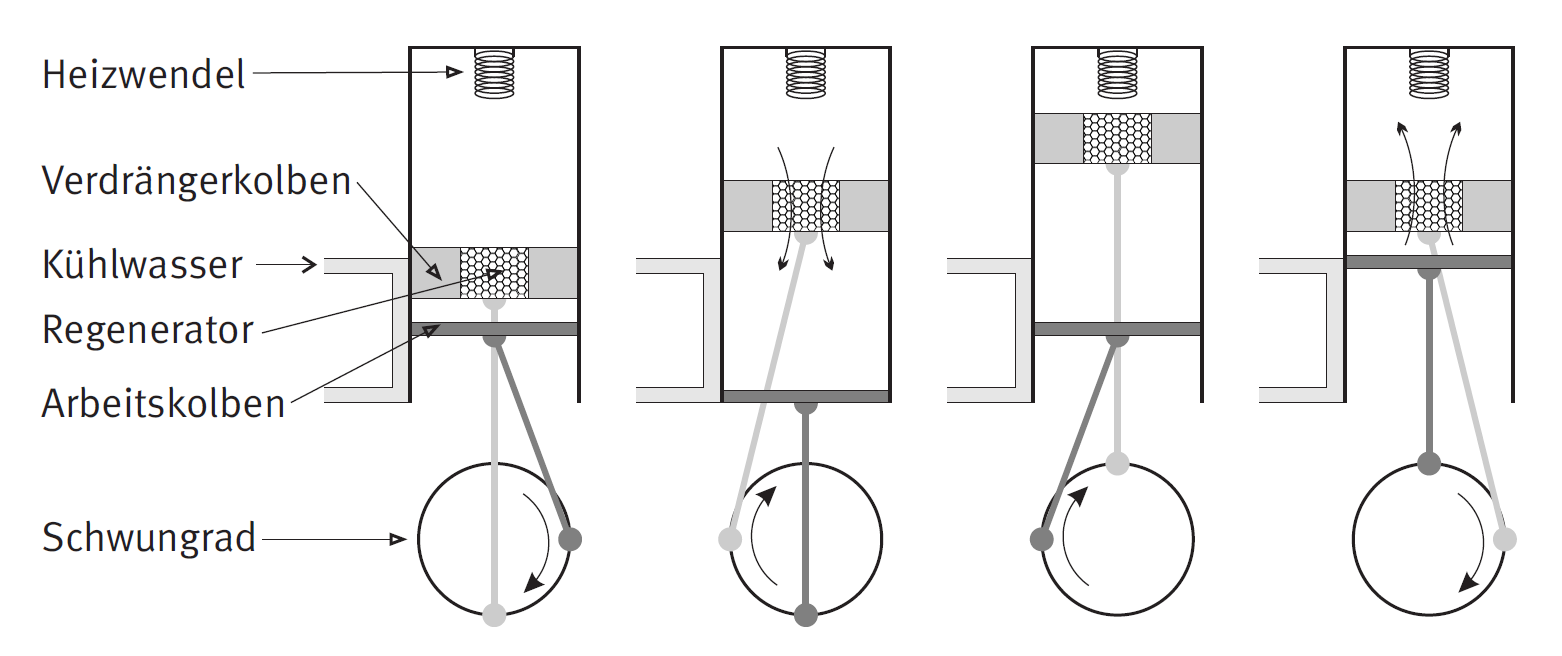
\includegraphics[width=\textwidth]{Aufbau.png}
			\caption{Darstellung der Takte des Stirling-Motors. Isotherme Expansion, isochore Abkühlung, isotherme Kompression und isochore Erwärmung (von links nach rechts).\cite{WWU}}
			\label{fig:Aufbau}	
		\end{figure}
				
	\subsection{Unsicherheiten}
	
		Jegliche Unsicherheiten werden nach GUM bestimmt und berechnet\footnote{Die Gleichungen dazu finden sich im Anhang unter \ref{fig:GUM_combine}, \ref{fig:GUM_formula}.}.
		Für die Unsicherheitsrechnungen wurde die Python Bibliothek "uncertainties" herangezogen, welche den Richtlinien des GUM folgt.
	
		Für digitale Messungen wird eine Unsicherheit von $u(X) = \frac{\Delta X}{\sqrt{3}}$ angenommen, bei analogen eine von $u(X) = \frac{\Delta X}{\sqrt{6}}$.
		
		\begin{description}
			\item[Abtastrate] Für die zeitliche Abtastrate des Messprogramms wurde eine Unsicherheit entsprechend der Abtastfrequenz mit $\Delta t = \frac{1}{f}$ gewählt.
			Die Messung erfolgt digital.
			
			\item[Position] Bei der Positionsbestimmung wurde durch die Schrittweite der Daten eine Unsicherheit von $\Delta x = \SI{0.1}{\milli\meter}$ festgelegt.
			Die Messung ist digital.
			
			\item[Stoppuhr] Die Unsicherheit setzt sich aus der analogen Reaktionszeit und der digitalen Stellengenauigkeit nach \ref{fig:GUM_combine} zusammen.
			Die Zeit kann beim Messprozess gut abgeschätzt werden, da der Füllstand des Messzylinder linear zunimmt, also ist die Reaktionszeit auf $\Delta t_1 = \SI{0.1}{\second}$ abgeschätzt.
			Die Stoppuhr kann zwei Nachkommastellen angeben, also ist $\Delta t_2 = \SI{10}{\milli\second}$.
			
			\item[Messzylinder] Das Volumen des Zylinders ist in \SI{1}{\milli\liter} unterteilt.
			Es wird analog abgelesen.
			Also folgt $\Delta V = \SI{1}{\milli\liter}$.
			
			\item[Pipette] Die Pipette, mit welcher die Probemenge bestimmt wurde, hatte auf \SI{1}{\milli\liter} Einhundert Unterteilungen und wurde ebenfalls analog abgelesen.
			Dementsprechend folgt $\Delta V = \SI{0.01}{\milli\liter}$.
			
			\item[Thermometer] Sowohl das Programm, als auch das manuelle Thermometer konnten auf eine Nachkommastelle genaue Angaben machen.
			Beide sind digital.
			Es ergibt sich die Unsicherheit $\Delta T = \SI{0.1}{\celsius}$.
		\end{description}
		
		In Diagrammen mit vielen Messpunkten wurden aus Gründen der Übersichtlichkeit nicht für jeden Punkt Unsicherheitsbalken gezeichnet.
		
\section{Durchführung und Datenanalyse}	
	\begin{figure}[ht]
		\centering
		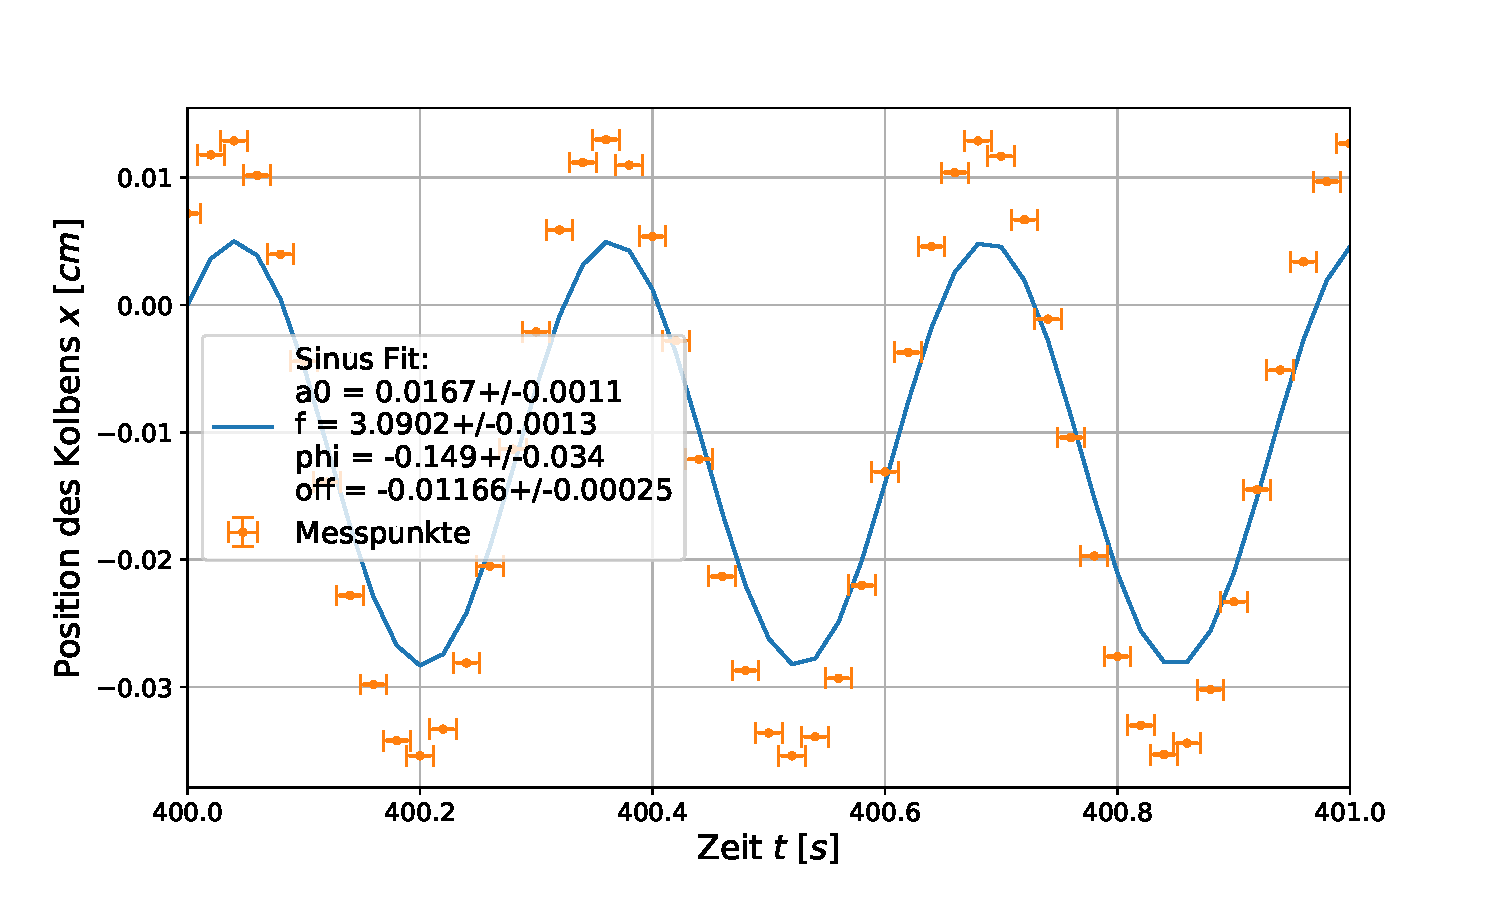
\includegraphics[width=\textwidth]{data/Position.pdf}
		\caption{Sinus-Fit zur Rotation des Motors. Der Parameter $f$ ist die gefittete Frequenz.}
		\label{fig:Frequenz}	
	\end{figure}
	Damit der Motor mit einer Frequenz von $\approx$ \SI{3}{\hertz} arbeiten konnte, wurde seine Rotation aufgenommen und das Zeitbild am Computer fourier-transformiert, sodass eine passende Frequenz über Geschwindigkeitsänderung des Motors festgelegt werden konnte.
	Diese Messung ist in Abb. \ref{fig:Frequenz} mit einem Sinus-Fit dargestellt.
	Aus der FFT folgte eine Frequenz von ca. \SI{3,1}{\hertz}, welche durch den Fit bestätigt wurde.
	Für die weiteren Berechnungen wird die gefittete Frequenz verwendet.
	
	Zur Bestimmung der Reibungsarbeit wurde zunächst der Zylinderkopf des Stirling-Motors abgenommen und die Temperatur $T_{Abfluss,0} = \SI{24,5+-0,03}{\celsius}$ des Kühlwassers an diesem gemessen.
	Dann  wurde der Motor als Wärmepumpe in Betrieb genommen.

	Ab dem Punkt, an dem die Temperatur des Kühlwassers sich nicht mehr änderte, bei $T_{Abfluss} = \SI{25,0+-0,03}{\celsius}$, wurde der Volumendurchfluss an dem Kühlwasserreservoir gemessen.
	Daraus ergab sich eine Zeit $t_{MZ} = \SI{11,47+-0,003}{\second}$ für $V_{MZ} = \SI{50+-0,2}{\milli\liter}$ (MZ steht für Messzylinder).	
	Der Massendurchfluss ergibt sich aus:
	\begin{equation} % massenstrom des Kühlwassers [masse pro zeit]
		\dot{M} = \rho \frac{V_\text{MB}}{t_\text{MB}}.
	\end{equation} % rho ist dichte, V ist volumen des Messbechers, t ist Füllzeit des volumens
	Dabei ist $\rho$ die Dichte des Wassers.
	
	Allgemein gilt für das System:
	\begin{equation} \label{eq:W}% absolute Leistung der Maschine, ist dW < 0 so wird Energie aufgenommen, ist dW > 0 so wird Energie abgegeben/Arbeit von der Maschine geleistet; da wir hier Wärmepumpe/Kältemaschine haben ist dW < 0 und der Motor gibt Energie in das System ein
		\dot{W} = \dot{Q}_1 - \dot{Q}_2 + \dot{W}_\text{R},
	\end{equation} % Q_1 ist Wärme des Kühlwassers(negativ)[siehe (3)], Q_2 ist Wärme der Probe/gemessene Temperatur (4) -> Wärmeänderung(Kältemaschine: positiv, Wärmepumpe: negativ)
	wobei $W_\text{R}$ der gesuchten Reibungsarbeit entspricht.
	Aufgrund des linearen Verhaltens:
	\begin{equation} % Reibungswaerme pro Zeit(ist negativ, weil Reibungsarbeit geleistet wird)
		\dot{W}_\text{R} = \dot{Q}_\text{R} = c \dot{M} (T_\text{Reservoir} - T_\text{Abfluss}),
	\end{equation} % c ist spez. Wärme (von wasser), M wie oben, T_zu ist zulaufende Temperatur, T_ab ist ablaufende Temperatur
	lässt sich die zeitliche Änderung als Reibungsänderung pro Zeit darstellen.
	Die oben genannten Größen $Q_{1/2}$ entsprechen der von dem System aufgenommenen bzw. abgegebenen Wärme und $c$ entspricht der spezifischen Wärme des Wassers.
	Über die Gleichungen
	\begin{equation} % analog dazu Wärme von kalt, warm machen
		\dot{Q}_1 = c \dot{M} (T_\text{Reservoir} - T_\text{Abfluss})
	\end{equation} % T_zu ist zulaufende Temperatur, T_ab ist ablaufende Temperatur bei kalt/warm machen
	und
	\begin{equation} \label{eq:Q2} % Wärmeänderung der Probe pro Zeit
		-\dot{Q}_2 = c \rho V_\text{Probe} \dd{T}
	\end{equation} % V_P = Volumen der Probe; dT Steigung des Graphen bei Raumtemp
	sind alle Größe der Systemgleichung beschrieben.
	Für $c$ und $\rho$ werden die Literaturwerte des NIST\cite{NISTwater} herangezogen.
	$V_\text{Wasser}$ beschreibt das Volumens der Probe in dem Zylinderkopf, welche für die Berechnung der Reibungsarbeit jedoch wegfällt.
	Einsetzen der Messwerte liefert eine Reibungsleistung von \SI{9.1+-1.5}{\joule\per\second} bzw. \SI{3.0+-0.5}{\joule} pro Umdrehung.	
	
	\begin{figure}[ht]
		\centering
		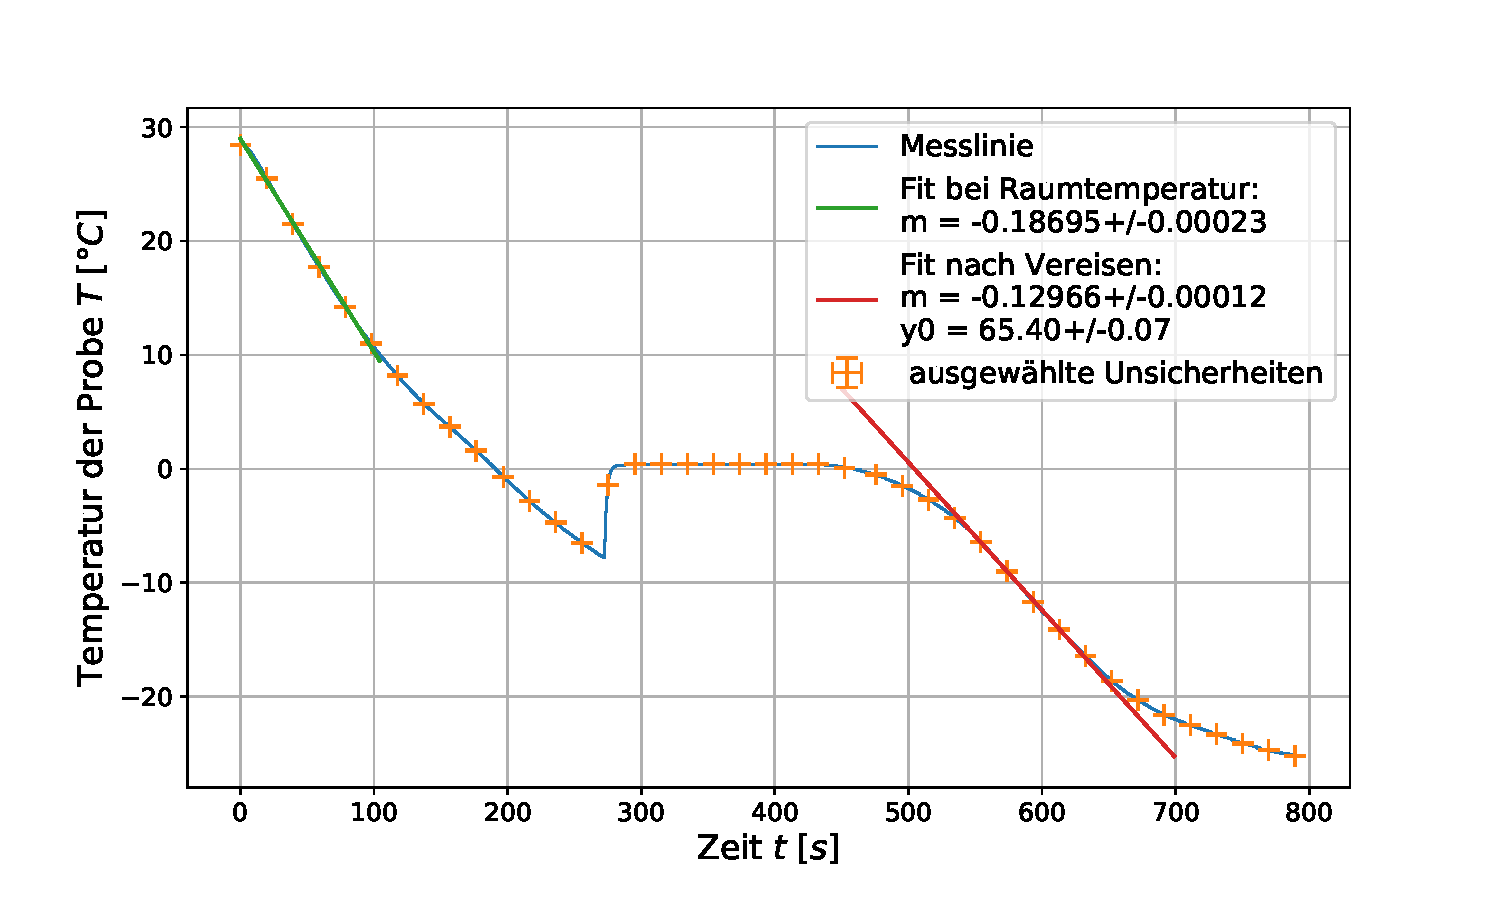
\includegraphics[width=\textwidth]{data/kalt_machen.pdf}
		\caption{Temperatur-Verlauf des Wassers bei der Kältemaschine.}
		\label{fig:Kältemaschine}	
	\end{figure}
	Nun zu der Verwendung des Motors als Kältemaschine.
	Dazu wurde der Zylinderkopf wieder verschraubt und \SI{1}{\milli\liter} destilliertes Wasser in das daran befestigte Reagenzglas gefüllt.
	Abbildung \ref{fig:Kältemaschine} zeigt den aufgenommen Verlauf der Temperatur des Wassers mit einer Abtastrate von \SI{10}{\hertz}.
	\begin{figure}[ht]
		\centering
		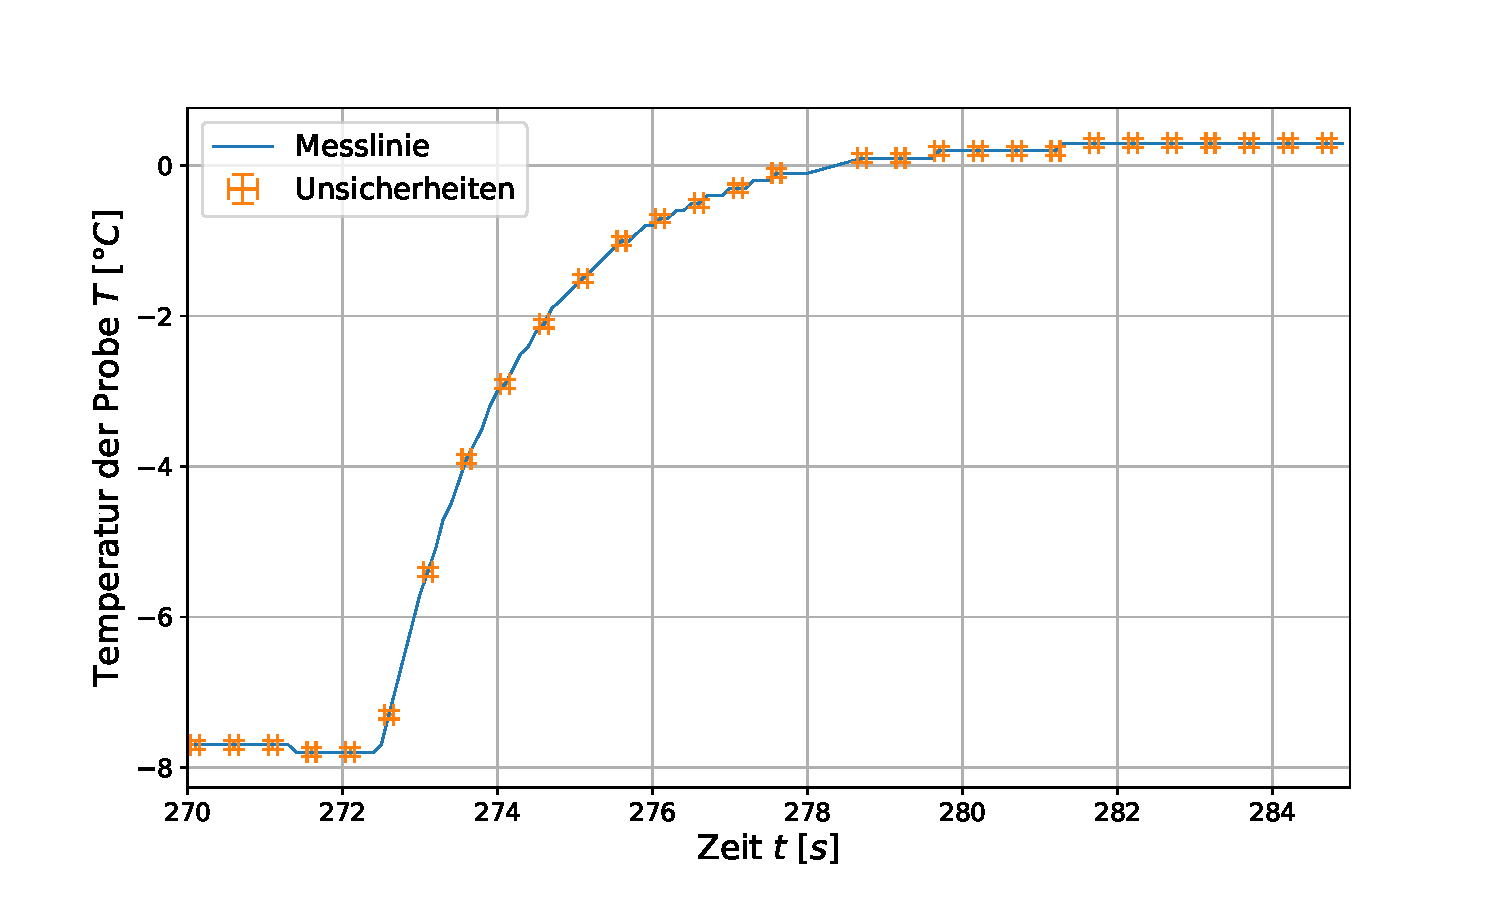
\includegraphics[width=\textwidth]{data/kalt_sprung.pdf}
		\caption{Genauere Darstellung des Sprungs in der Temperaturkurve der Kältemaschine.}
		\label{fig:KaltSprung}	
	\end{figure}

	Auffällig daran ist der schlagartige Anstieg bzw. Sprung von ca. \SI{-8}{\celsius} auf ungefähr \SI{0}{\celsius} und der darauf folgende konstante Bereich, bis die Temperatur wieder anfängt zu sinken.
	Der Sprung wird in Abbildung \ref{fig:KaltSprung} deutlicher dargestellt.
	Nachdem eine Temperatur  von ca. \SI{-26,7}{\celsius} erreicht wurde, wurde zudem eine Messung der Temperatur des abfließenden Kühlwassers $T_\text{Abfluss} = \SI{26,6+-0,03}{\celsius}$ und der im Reservoir $T_\text{Reservoir} = \SI{25,3+-0,03}{\celsius}$ durchgeführt.
	Die Schmelzwärme $Q_\text{G}$ bei dem Gefriervorgang des Wassers lässt sich über 
	\begin{equation} % Schmelzwärme gefrieren
		Q_\text{G} = Q_2 (t_2 - t_1) + Q
	\end{equation} % t_1 Anfangszeitpunkt des Gefrierens nach kristallisieren(Stufe); t_2: Endzeitpunkt (durch linearisierung des theoretisch homogenen kühlprozesses bestimmt); Q von vorher(7); Q_2 beim gefrieren
	mit
	\begin{equation} \label{eq:Q} % Wärme beim Kristallisieren des Eises
		Q = c \rho V_\text{Probe} (T_2 - T_1)
	\end{equation} % T_2: Temperatur kurz nach dem Gefrierens; T_1: Temperatur kurz vor dem Gefrieren
	bestimmen.
	Dabei sind $t_{1/2}$ die Zeiten am Anfang und Ende des Gefrierprozesses und $T_{1/2}$ die Temperaturen kurz vor und direkt nach dem Sprung.
	Es ist zu beachten, dass $t_2$ durch Extrapolation des Graphen einige Zeit nach dem erneuten abfallen der Temperatur ermittelt wurde.
	Das inhomogene Abkühlen der Probe, welches durch die Kühlung von Außen auftritt, soll somit umgangen werden.
	
	$Q_2$ folgt aus Gl. \ref{eq:Q2}.
	Einsetzen führt zu einer Schmelzwärme $Q_\text{G} = \SI{215.8+-1.2}{\joule\per\gram}$ 
	Für die Kühlleistung $\varepsilon$ dient folgender Zusammenhang:
	\begin{equation} \label{eq:eps} % kühlleistung/heizleistung
		\varepsilon = \frac{\abs{Q_2}}{\abs{W}}
	\end{equation} % Q_2 (4), W (5)
	Dabei sind $Q_2$ und W den Gleichungen \ref{eq:Q2} und \ref{eq:W} zu entnehmen.
	Aus dieser Messung folgt $\varepsilon = 0,0233\pm 0,0015$ für die Kühlleistung.
	
	\begin{figure}[ht]
		\centering
		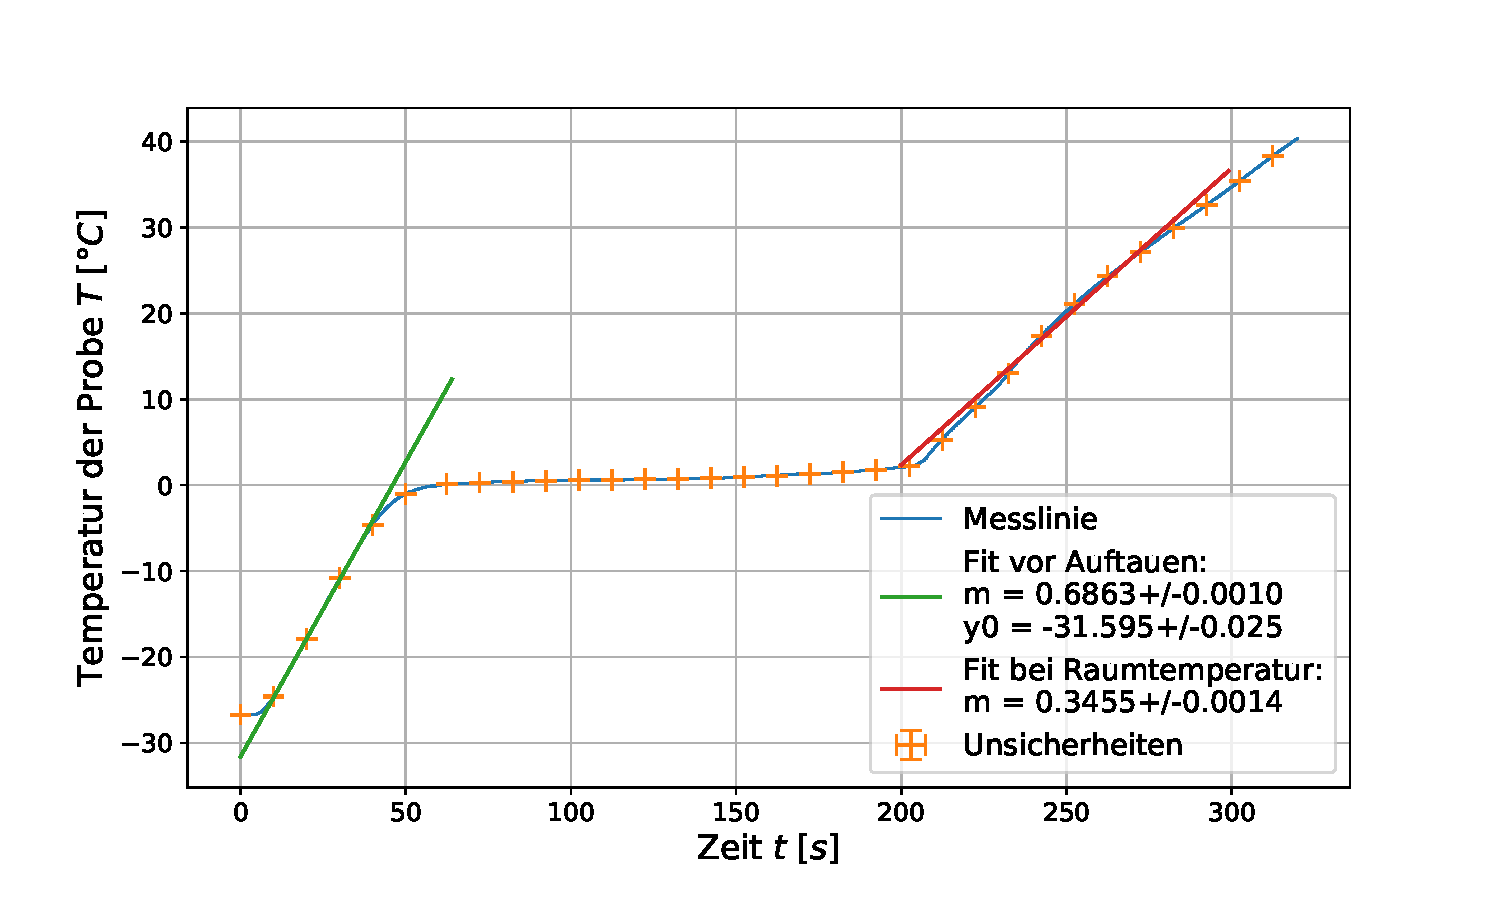
\includegraphics[width=\textwidth]{data/warm_machen.pdf}
		\caption{Temperatur-Verlauf des Wassers bei der Wärmepumpe.}
		\label{fig:Wärmepumpe}	
	\end{figure}
	Analog zur Kältemaschine verlief die Untersuchung der Wärmepumpe. 
	Die Temperaturkurve des Wassers bei diesem Vorgang ist in Abb. \ref{fig:Wärmepumpe} aufgetragen.
	Diese verzeichnet einen der Kältemaschine ähnlichen Verlauf.
	Hier tritt jedoch kein Sprung auf, die Temperatur bleibt dennoch bei ungefähr \SI{0}{\celsius} für einige Zeit konstant, bevor sie wieder ansteigt.
	Auch hier wurde erneut eine Messung der Temperatur des abfließenden Kühlwassers $T_\text{Abfluss} = \SI{25,5+-0,03}{\celsius}$ und der im Reservoir $T_\text{Reservoir} = \SI{25,5+-0,03}{\celsius}$ durchgeführt.
	Dies geschah bei der Temperatur des Wassers von ca. $T_\text{Probe} = \SI{40,4}{\celsius}$.
	Die Berechnung der Heizleistung aus dieser Kurve verlief analog zu der bei der Kältemaschine vgl. Gl. \ref{eq:eps}.
	Dür diese ergibt sich $\varepsilon = 0,19\pm 0,05$.
	Für eine erneute Bestimmung der Schmelzwärme, dieses mal jedoch bei dem Schmelzprozess, dient folgende Formel:
	\begin{equation} % Schmelzwärme schmelzen (Q_S = Q_G)
		Q_\text{S} = -Q_2 (t_2 - t_1).
	\end{equation} % das gleiche nur ohne Q, weil keine stufe; *-1 weil Energie reingesteckt wird
	Auch hier ist $Q_2$ wieder der Gl. \ref{eq:Q2} zu entnehmen und die Zeiten wurden ggf. extrapoliert.
	Dies führt zu einem Ergebnis der Schmelzwärme von ebenfalls $Q_\text{S} = \SI{215.8+-1.2}{\joule\per\gram}$.
	Letztlich sollte für diese Messung noch die spezifische Wärme von Eis bestimmt werden.
	Diese ergibt sich aus:
	\begin{align}
		\dot{Q} &= c_\text{Eis} m_\text{Probe} \dd T\\
		\Leftrightarrow c_\text{Eis} &= \frac{\dot{Q}}{m_\text{Probe}\dd T}
	\end{align} % c_Eis spez. Wärme Eis; m_P masse Probe; dQ wie oben
	mit
	\begin{equation}
		m_\text{Probe} = \rho V_{Probe}.
	\end{equation} % die masse der probe ändert sich nicht, auch wenn es zu eis wird
	Über Gl. \ref{eq:Q} ergibt sich hierfür: $c_\text{Eis}=\SI{2.108+-0.010}{\joule\per\gram\per\kelvin}$.
	
\section{Diskussion}
	
	Nun stellt sich die Frage, ob die Ziele der Untersuchung erreicht wurden.
	Dazu wird zunächst betrachtet, ob die Werte für Reibungsarbeit und Heiz- bzw. Kühlleistung physikalisch sinnvoll sind.
	Der ermittelte Wert für die Reibungsarbeit entspricht \SI{3.0+-0.5}{\joule} pro Umdrehung, welcher in einer denkbaren Größenordnung liegt.
	Für Heiz- und Kühlleistung ergaben sich $\varepsilon = 0,0233\pm 0,0015$ und $\varepsilon = 0,19\pm 0,05$.
	Bei diesen %TODO wie gut?
	
	Der Sprung bei dem Verlauf der Temperatur und der darauffolgende konstante Bereich bei der Kältemaschine lassen sich über die Schmelzwärme erklären.
	Diese Wärme wird benötigt um von dem festen Zustand in den flüssigen zu wechseln.
	Umgekehrt wird diese Wärme freigelassen, wenn der Wechsel von flüssig nach fest stattfindet.
	Dies geschieht nicht direkt bei \SI{0}{\celsius}, sondern erst nachdem sich Kristalle in der Flüssigkeit gebildet haben, welche sich schlagartig vermehren und zu dem Gefrieren der Flüssigkeit führen.
	Bis zur kompletten Kristallisierung bleibt die Temperatur bei ungefähr \SI{0}{\celsius} und fällt danach wieder ab.
	Bei der Wärmepumpe hingegen muss die erforderliche Schmelzwärme dem Eis hinzu geführt werden, weswegen auch hier der Temperaturverlauf für einige Zeit konstant bleibt. 
	Dass die ermittelten Werte für die Schmelzwärme aus beiden Messungen exakt übereinstimmen, $Q_\text{G} = Q_\text{S} = \SI{215.8+-1.2}{\joule\per\gram}$, ist zwar für eine Messung hervorragend, jedoch weichen diese Ergebnisse um ca. 35,4\% von dem Literaturwert\cite{Toolbox} ab.
	Diese Abweichung ist zu groß, als das hier von einer genauen Übereinstimmung berichtet werden kann.
	Bei der spezifischen Wärme von Eis hingegen wurde ein Wert von $c_\text{Eis}=\SI{2.108+-0.010}{\joule\per\gram\per\kelvin}$ bestimmt. 
	Dieser Wert liegt exakt auf dem Literaturwert\cite{Toolbox} von $\SI{2.108}{\joule\per\gram\per\kelvin}$, weswegen zumindest an dieser Stelle eine genaue Übereinstimmung vorliegt.
	